%%%%%%%%%%%%%%%%%%%%%%%%%%%%%%%%%%%%%%%%%%%%%%%%%%%%%%%%%%%%%%%%%%%%%%%%%%%%%%%%%%%%%%%%%%%%%
%%									Chapitre 6												%
%%%%%%%%%%%%%%%%%%%%%%%%%%%%%%%%%%%%%%%%%%%%%%%%%%%%%%%%%%%%%%%%%%%%%%%%%%%%%%%%%%%%%%%%%%%%%

\chapter{Techniques de quantification et {\em Arterial Spin labeling}}
\label{chap:asl}
	\minitoc

%%%%%%%%%%%%%%%%%%%%%%%%%%%%%%%%%%%%%%%%%%%%%%%%%%%%%%%%%%%%%%%%%%%%%%%%%%%%%%%%%%%%%%%%%%%%%

L’Arterial Spin Labeling (ou ASL) est une technique sans injection de mesure de la perfusion cérébrale basée sur deux acquisitions du volume d’intérêt avec et sans marquage radiofréquence à 180° des protons artériels. La différence de ces deux images élimine la composante statique du signal pour ne mettre en évidence que la perfusion.

Nous allons passer en revue les méthodes d’acquisition et de quantification disponible pour mettre en oeuvre cette technique, avant de nous concentrer sur les limitations et les problèmes méthodologiques.
%%%
%%%
%%%
\section{Acquisition}
Du point de vue de l’acquisition les différentes méthodes disponibles se distinguent par le décours de la cinétique du marquage des protons. On distingue principalement des techniques de marquage continu (CASL) et le marquage pulsé (PASL).

Présentons tout d’abord le marquage continu (CASL). Cette méthode développée par Williams et collaborateurs en 1992  (\cite{Detre1992},~\cite{Williams1992}) consiste à appliquer une impulsion radiofréquence pendant 2 à 4 secondes de façon continue au niveau du plan de marquage, lors de l’application d’un gradient de champs magnétique dans la direction du flux (\cite{Ferre2011}). L’image obtenue dispose d’un haut rapport signal sur bruit mais a en contrepartie deux inconvénients inhérents au marquage continu. Ces inconvénients sont d’une part la présence d’un transfert d’aimantation (MT) et d’autre part un dépôt d’énergie plus important dans les tissus. Le transfert d’aimantation correspond à une contamination du signal au voisinage des protons marqués et va avoir pour conséquence de réduire ce signal et donc d’affecter la mesure de débit, mais aussi de complexifier l’acquisition d’images multi-coupes. Pour limiter ce phénomène spécifique à l’image marquée, un marquage distal est réalisé dans l’acquisition contrôle elle-même afin d’y produire le même effet de transfert d’aimantation.

Pour réduire la durée d’application des impulsions, une nouvelle approche a récemment été développée, l’ASL pseudo-continu (pCASL). A la place d’une seule et longue impulsion, 1000 impulsions ou plus sont appliquées à une fréquence d’une impulsion par milliseconde (\cite{Dai2008}). Le marquage est aussi long que dans la méthode continue, mais conduit à une bien meilleure efficacité par réduction de des effets de transfert d’aimantation, le tout en étant compatible avec les systèmes modernes d’antennes. C’est à l’heure actuelle la séquence recommandée en imagerie clinique(\cite{Alsop2014}) bien qu’elle ne soit pas, pour le moment, fournie en version « standard » par tous les constructeurs.

%%%
\begin{figure}[!t]
\centering
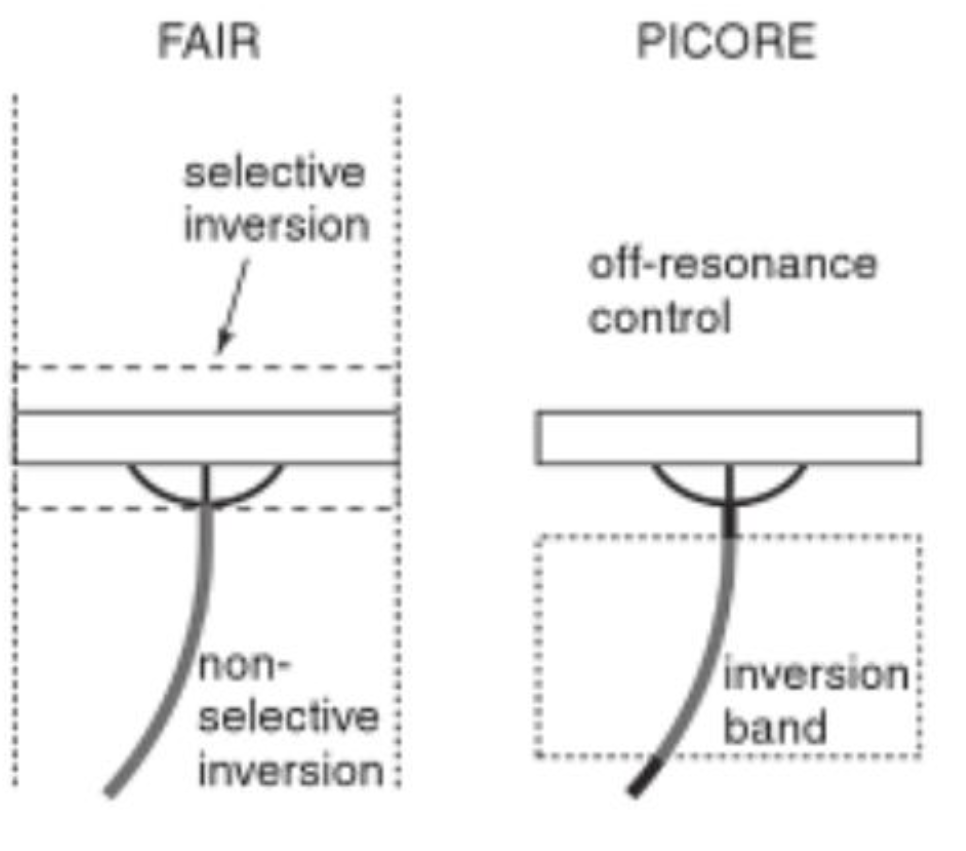
\includegraphics[width=5cm]{5_1_fair_picore}
\caption{Différence entre le marquage ASL FAIR et PICORE.}
\label{fig:5_1_fair_picore}	
\end{figure}
Les méthodes d’ASL pulsées (PASL) en revanche sont devenues les plus communes car disponibles en version commerciale chez les principaux constructeurs (\cite{Petersen2006}). Contrairement au CASL, où le sang est inversé en continu dans une zone fine et bien définie, les approches de PASL, se basent sur l’utilisation d’impulsions radiofréquence courtes sur de grandes régions à proximité du cerveau. Parmi les séquences de PASL on peut distinguer deux groupes en fonction de la position de la zone de marquage par rapport aux coupes : les méthodes symétriques et les méthodes asymétriques (\cite{Petersen2006}). Les méthodes symétriques de type FAIR (Flow Alternating Inversion Recovery) utilisent une impulsion d’inversion non sélective lors du contrôle à laquelle est ajoutée un gradient de sélection de coupe pour le marquage (\cite{Wong1997}).  Les méthodes asymétriques, comme la séquence PICORE (proximal inversion with a control for off-resonance effects), utilisent une zone de marquage placée à 1 à 2 cm en amont du volume d’intérêt. Dans cette séquence, le marquage est réalisé en utilisant une impulsion d’inversion sélective à proximité de la zone à imager. L’acquisition contrôle est constituée de la même impulsion radiofréquence, mais appliquée hors résonance de coupe et sans gradients allumés, si bien qu’aucune inversion effective n’est réalisée (\cite{Wong1997},~\cite{Buxton2009}) (Figure~\ref{fig:5_1_fair_picore}). Les deux approches offrant des résultats similaires (\cite{Cavusoglu2009}).

%%%
\begin{figure}[!t]
\centering
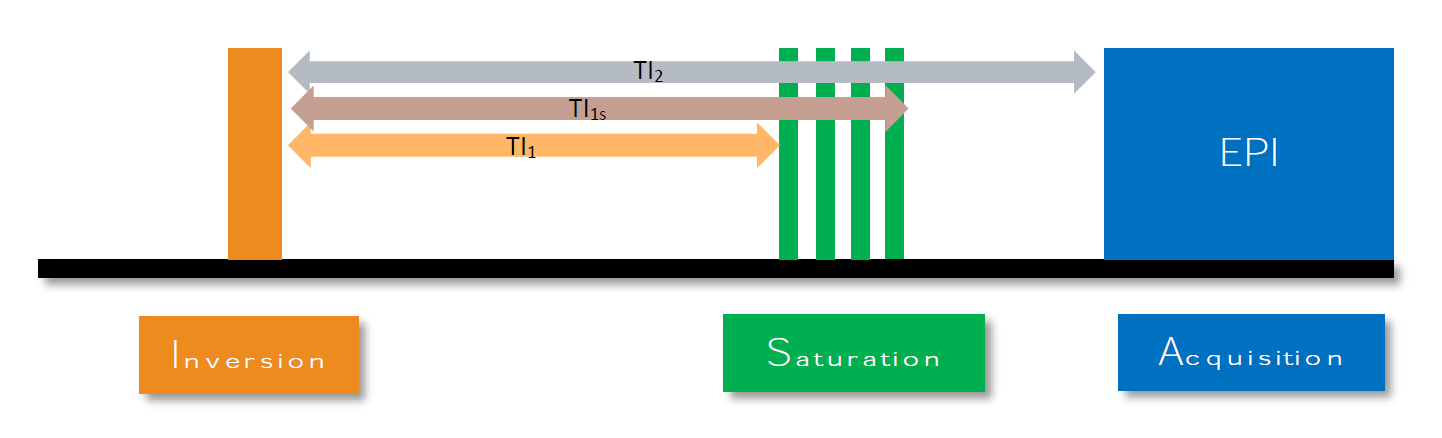
\includegraphics[width=12cm]{5_2_q2tips}
\caption{Séquence PICORE-Q2TIPS.}
\label{fig:5_2_q2tips}	
\end{figure}
Des optimisations de la séquence ont par la suite été réalisées pour réduire la sensibilité au temps de transit comme la séquence Q2TIPS (\cite{Luh1999}, voir figure~\ref{fig:5_2_q2tips}). Ainsi ont été rajoutées à cette séquence des impulsions de saturation (90°) périodiques après un temps T$_1$ (en général 700 ms) permettant de délimiter précisément la largeur temporelle du bolus marqué. On définit ainsi la durée du bolus (T$_{I_1}$), la fin des impulsions de saturation (T$_{I_{1s}}$) et le temps d’inversion (T$_{I_2}$).

Du fait du rapport signal sur bruit faible et de la nécessité de répéter les acquisitions contrôles et label, le choix de la technique d’acquisition des images est très important. Ainsi l’echo planar imaging (EPI) est le plus souvent utilisé. Il autorise une acquisition rapide limitant les artefacts de mouvement et dispose d’un bon rapport signal sur bruit. L’inconvénient de cette séquence est qu’elle peut présenter des distorsions dans les régions de forte susceptibilité magnétique. 

Afin d’améliorer la qualité des images, des séquences 3D ont été développées. Il est possible d’utiliser des séquences single-shot 3D combinant écho de gradient et spin écho (GRASE,~\cite{Gunther2005}). Ces nouvelles séquences permettent d’aboutir à des images mieux résolues, présentant un meilleur rapport signal sur bruit et donc nécessitant moins de répétitions. De plus il devient possible d’utiliser de multiples impulsions d’inversion non sélectives, appelées « background suppression pulses », neutralisant le signal des tissus stationnaires sans affecter le sang marqué, ce qui améliore la qualité de l’image. Enfin grâce aux antennes en réseau phasé, ces séquences bénéficient de l’imagerie parallèle pour réduire la durée d’acquisition, ce qui autorise les protocoles multi temps d’inversion en une durée raisonnable (4 à 5 min).

%%%
\begin{figure}[!t]
\centering
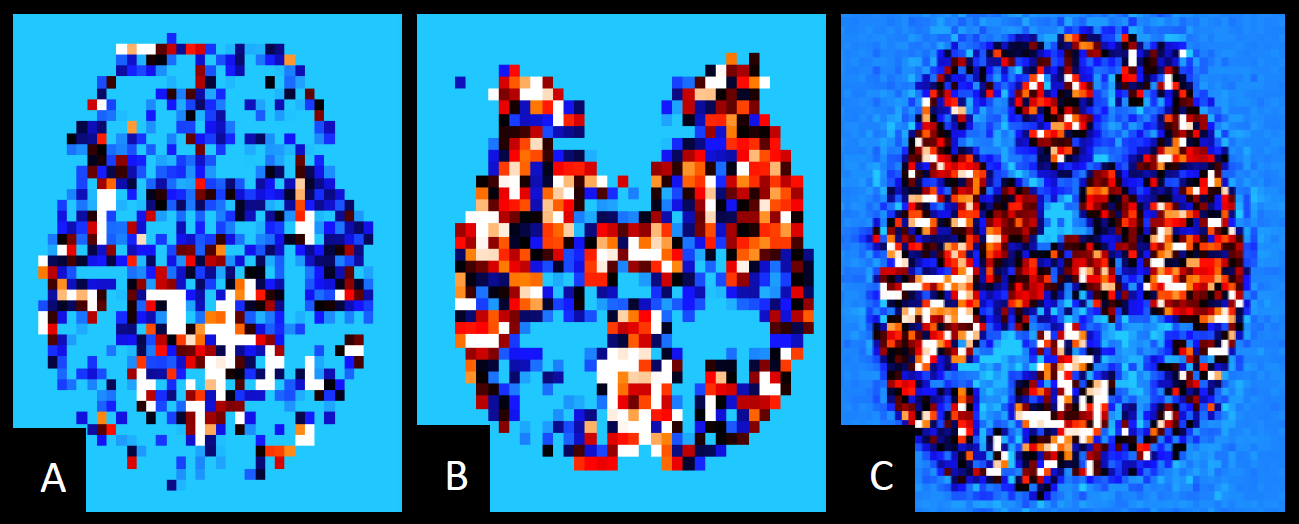
\includegraphics[width=10cm]{5_3_exemple_asl}
\caption{Exemple d'images de perfusion d’ASL 2D (PICORE-Q2TIPS) à 1.5T (A) et 3T (B) et d’ASL 3D à 3T (C).}
\label{fig:5_3_exemple_asl}	
\end{figure}
Il est bon pour finir de noter aussi l’importance de l’intensité du champ magnétique, dont l’augmentation permet d’améliorer significativement la qualité de l’ASL (\cite{Golay2006}) (Figure~\ref{fig:5_3_exemple_asl}). En effet, le rapport signal sur bruit augmente et le $T_1$ des tissus et donc le temps de marquage des protons également.
%%%
%%%
%%%
\section{Quantification}
La différence ($\Delta$M) images contrôle – images marquées permet d’obtenir une cartographie pondérée en perfusion. Le passage à une valeur absolue quantitative de la perfusion nécessite un modèle qui incorpore le temps de transit, le temps T$_1$ du tissu, le temps T$_1$ et la magnétisation du sang à l’équilibre (M$_0$), la densité de protons et bien entendu les paramètres d’acquisition.

Le modèle le plus simple proposé (modèle à un compartiment) a été dérivé des équations de Bloch (\cite{Bloch1946}) et repose sur plusieurs hypothèses (\cite{Petersen2006},~\cite{Parkes2005}). Tout d’abord le sang marqué est entièrement délivré à la zone à imager par simple transport dans la circulation. D’autre part les protons marqués du sang sont considérés comme un traceur diffusible, ce qui permet l’échange de magnétisation avec les spins du parenchyme cérébral. Le temps d’inversion est choisi de sorte à correspondre exactement à l’arrivée du sang marqué dans la zone à imager : l’élimination du marquage est négligeable au moment de l’acquisition. Par contre le sang marqué a été complètement éliminé avant les acquisitions suivantes. Enfin on suppose les effets de volume partiels négligeable : les différents sous compartiments du parenchyme (matière grise, matière blanche) possédant potentiellement des T$_1$ différents ne sont pas distingués.

Dans ce modèle la magnétisation des spins de la zone marquée est inversée au temps zéro et relaxe selon le temps caractéristique T$_1$ qui est celui du sang (T$_1$=T$_{1B}$). Lorsque les spins d’eau marqués échangent avec les spins de l’eau du parenchyme cérébral dans le lit capillaire, le temps de relaxation T1 des spins marqués passe du T$_{1B}$ au T$_1$ du tissu (T$_{1t}$,~\cite{Luh1999}). Pour une séquence d’ASL pulsée la modélisation physique montre alors qu’on peut obtenir le débit sanguin cérébral via la formule (\cite{Wang2003}) :
\begin{equation}
\label{eq:debit}
CBF\,=\,\frac{\lambda\,\Delta M}{2\;\alpha\,M_{0\alpha}\,T\,I_1\,e^\frac{-T I_2}{T_{1A}}}.
\end{equation}
Dans cette formule $\Delta$M est la différence moyenne entre l’image contrôle et l’image marquée
dans le voxel d’intérêt ; $\lambda$ est le coefficient de partage des eaux entre sang et tissu, défini comme le
ratio de la quantité d’eau par gramme de tissu et de la quantité d’eau par millilitre de sang ; $T_{1a}$ est le
temps de relaxation longitudinal du sang ; $\alpha$ est l’efficacité de l’inversion ; enfin $M_{0a}$ la magnétisation
du sang à l’équilibre. On obtient ainsi une mesure du débit sanguin cérébral en millilitres par 100
grammes de tissu par min (ml/100g/min).

Afin de mesurer la magnétisation du sang à l’équilibre, une acquisition additionnelle doit être
réalisée avec un temps de répétition très long (appelée $M_0$) dans laquelle il faut extraire la valeur dans
un voxel ne contenant que du sang. Cependant, du fait de la mauvaise résolution, il est très difficile de
trouver un tel voxel. La magnétisation du sang doit donc être estimée à partir de voxels contenant
d’autres tissus. Çavuşo\u{l}u et al. (\cite{Cavusoglu2009}) ont réalisé une revue des méthodes permettant de substituer au
paramètre global $M_{0a}$
les magnétisations $M_0$ soit de la matière blanche, soit du liquide
céphalorachidien, ou encore du tissu local (LT). Il est ainsi possible d’estimer $M_{0a}$ via l’Équation :
\begin{equation}
M_{0a}\,=\,M_i\,R_{0i}\,e^{\bigl(\frac{1}{T_{2i}^{\ast}}-\frac{1}{T_2\ast}\bigr)}\,T_E
\end{equation}
avec $i$ le type de tissu (matière blanche, liquide céphalo rachidien ou tissu local), $R$ le ratio de signal
tissu – sang issue d’une image pondérée en densité de proton, $T_2^{\ast}$ le temps de relaxation transversal
du tissue et du sang et $T_E$ le temps d’écho. Le $M_{0i}$ utilisé correspond à la magnétisation moyenne
observée dans les tissus utilisés comme référence, sauf dans le cas de la méthode LT où $M_{0a}$ est
estimée en chaque voxel sur la base de l’intensité du voxel de l’image $M_0$.

Dans cette dernière méthode, la magnétisation est mise à l’échelle grâce au coefficient de
partition sang cerveau (« blood/brain partion coefficient ») $\lambda$ (avec $\lambda = M_{0T}/M_{0a}$). Cette méthode
permet par ailleurs de corriger automatiquement le profil de sensibilité spatial de l’antenne ce qui en
fait la méthode recommandée (\cite{Cavusoglu2009}).
%%%
%%%
%%%
\section{Limitations}
%%%
%%%
\subsection{Le modèle utilisé}
%%%
\begin{figure}[!t]
\centering
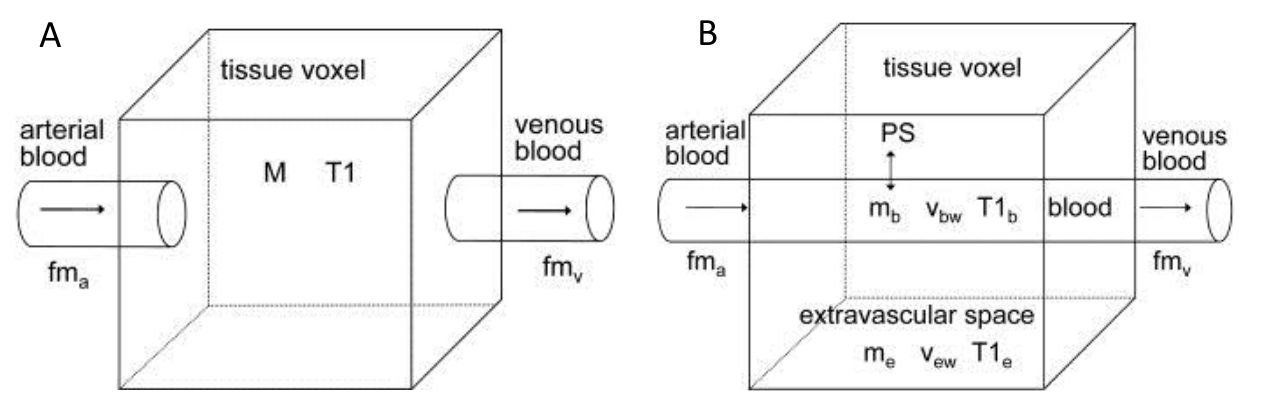
\includegraphics[width=10cm]{5_4_modeles_compartiments}
\caption{Modèle à un et deux compartiments. A) Modèle à un compartiment. Le sang marqué entre dans le voxel de tissu
avec une magnétisation $m_a$ et une perfusion $f$, et repart avec une magnétisation $m_z$. Le voxel dispose d’une magnétisation
$M$ et d’un temps de relaxation $T_1$. B) Modèle à deux compartiments avec une perméabilité restreinte. L’eau marquée est
échangée entre un compartiment sanguin et un compartiment extravasculaire via le mur capillaire via PS. Illustration issue
de~\cite{Parkes2005}.}
\label{fig:5_4_modeles_compartiments}	
\end{figure}
A l’aide des techniques précédentes, il est donc possible d’aboutir à une quantification du débit
sanguin cérébral. Néanmoins, les techniques d’ASL souffrent de quelques écueils. Le modèle
monocompartimental se recommande par sa simplicité et sa robustesse (\cite{Alsop2014}). Cependant, en réalité,
l’eau du sang marqué n’échange pas immédiatement avec l’eau extravasculaire, car elle reste un
certain temps dans le vaisseau avant de passer le mur capillaire vers l’espace extravasculaire. Pour
prendre en compte cela, d’autres modèles plus compliqués, à deux compartiments (Figure~\ref{fig:5_4_modeles_compartiments}) ont
été mis au point. Dérivés des modèles de perfusion injectés (\cite{Parkes2005}), ils intègrent les notions de
perméabilité et permettent ainsi d’accéder à de nouveaux paramètres.

%%%
%%%
\subsection{Le mouvement}
L’ASL requiert la soustraction de deux images acquises à différents temps pour récupérer le
signal d’intérêt qui ne représente que quelques pourcent du signal. Cette étape est très sensible au
mouvement qui peut dégrader significativement la qualité de l’image et induire d’importantes erreurs
dans l’estimation du débit sanguin cérébral. Deux pistes permettent de réduire ces artéfacts. Tout
d’abord au niveau de l’acquisition elle-même l’utilisation de séquences ultra-rapides telles que l’EPI ou
imagerie SPIRAL. Mais aussi au niveau du post-traitement des images l’utilisation d’outils de
réalignement standard (\cite{Friston2006}) ou dédiés à l’ASL (\cite{Wang2012}).
%%%
%%%
\subsection{Le temps de transit}
Que ce soit en CASL ou PASL, le sang marqué doit se déplacer de la zone de marquage à la
région d’intérêt. Ce déplacement se produit en un temps appelé temps de transit, $\delta$. Durant ce temps,
l’eau marquée se relaxe selon une constante de temps $T_{1a}$, ce qui induit une diminution du marquage
effectif dans la zone de mesure. Les méthodes récentes d’acquisition permettent néanmoins de limiter
ce problème en améliorant la qualité du marquage ou diminuant la distance de transit (Q2TIPS etc.). Il
reste néanmoins à la charge de l’utilisateur de sélectionner un temps d’inversion adapté au patient,
suffisamment long pour permette au bolus d’arriver dans la zone à imager, mais suffisamment court
pour éviter une perte du signal. Ce problème devient majeur avec des cohortes de plus d’une centaine
de patients lorsque le protocole contraint à n’utiliser qu’un seul et même temps d’inversion pour tous
les sujets (\cite{Deverdun2015}). Le développement des séquences multi-$T_I$ permet d’éviter ces problèmes en balayant
plusieurs temps d’inversion, ce qui autorise par ailleurs l’utilisation de modèles dédiés. Ceux-ci
permettant d’estimer plus précisément le débit tout en générant une cartographie des temps
d’arrivées du bolus (BAT) (\cite{Chappell2009}).
%%%
%%%
\subsection{Contamination vasculaire du signal}
Idéalement, tout le signal des protons marqués a été déposé dans les tissus lorsque l’image est
acquise. Cependant il est fréquent du fait de l’unicité du temps d’inversion qu’une partie résiduelle du
signal marqué soit encore contenue dans la vascularisation en amont des lits capillaires. Ce sang n’est
pas dans une zone d’échange avec le parenchyme et induit un biais sur l’évaluation de la différence de
magnétisation : il conduit à une surestimation du débit sanguin cérébral, introduisant des artéfacts
dans l’image identifiables sous forme de points clairs. Cette contamination vasculaire du signal
provient des vaisseaux traversant la zone d’intérêt pour perfuser d’autres territoires plus distaux. La
solution actuellement utilisée afin d’éliminer le signal de ces vaisseaux consiste à appliquer des
gradients bipolaires appelés « crusher » avant l’acquisition (\cite{Ye1997}). Il est néanmoins important de limiter
leur usage afin de ne pas induire une baisse trop importante du signal de perfusion.

%%%
%%%
\subsection{Effets de volume partiel}
\label{sec:volpar}
Les acquisitions rapides se font au détriment de la résolution. Ainsi les voxels ne sont que
rarement constitués d’un seul tissu. Un voxel typique contient plutôt un mélange de matière grise,
blanche et liquide céphalo rachidien en proportions variables. Or en termes de magnétisation, la
contribution au signal des différents tissus est différente. Le signal mesuré est en fait la moyenne du
signal issue de processus d’échanges entre les protons marqués et les protons de chacun de ces trois
tissus, et ceci dans des proportions variables selon les voxels. En toute rigueur, il faudrait introduire
dans le modèle les fractions de ces tissus dans le voxel d’intérêt que l’on peut obtenir via une segmentation. En l’absence de cette modélisation, on a une mauvaise estimation de la perfusion
cérébrale. Il est ainsi important de prendre en compte ces effets pour la quantification. Comment
prendre en compte ces effets pour la quantification ?

Les premières approches issues de l’imagerie PET consistaient simplement en l’application
d’un facteur de correction, sur la base de la segmentation des tissus en matière grise et matière
blanche, et en faisant l’hypothèse que la perfusion de la matière blanche correspond à 40 \% de celle
de la matière grise (\cite{Kim2012}). Asllani {\em et al.} ont proposé en 2008 un nouvel algorithme de correction des
effets de volume partiels dédié à l’ASL (\cite{Asllani2008}). Cette correction se base sur une formule simple qui décrit
la différence de signal mesurée comme étant une pondération de la contribution des différents tissus :
\begin{equation}
\label{eq:asllani}
\Delta M\,=\,P_{GM}\,\ast\,\Delta M_{GM}\,+\,P_{WM}\,\ast\,\Delta M_{WM}\,+\,P_{CSF}\,\ast\,\Delta M_{CSF},
\end{equation}
avec $\Delta M$ la différence image contrôle image marqué mesurée ; $P_{GM}$ , $P_{WM}$ , et $P_{CSF}$ les probabilités
postérieures obtenus par segmentation d’une image anatomique ; et $\Delta M_{GM}$ , $\Delta M_{WM}$  , et $\Delta M_{CSF}$  les
contributions propres au signal de la matière grise, matière blanche et liquide céphalorachidien. La
méthode repose ainsi sur l’extraction de ces contributions. Cependant, cette unique équation
contenant 3 inconnues, elle ne possède pas de solution unique. On fait alors l’hypothèse que la
perfusion reste constante dans un kernel local autour d’un voxel d’intérêt, de façon à générer un
ensemble d’équations possédant une solution unique. Il devient alors possible d’estimer $\Delta M_{GM}$ , $\Delta M_{WM}$  , et $\Delta M_{CSF}$ . Une fois cela réalisé les débits sanguins cérébraux partiels (propre à chaque tissu)
peuvent être obtenus.

\begin{figure}[!t]
\centering
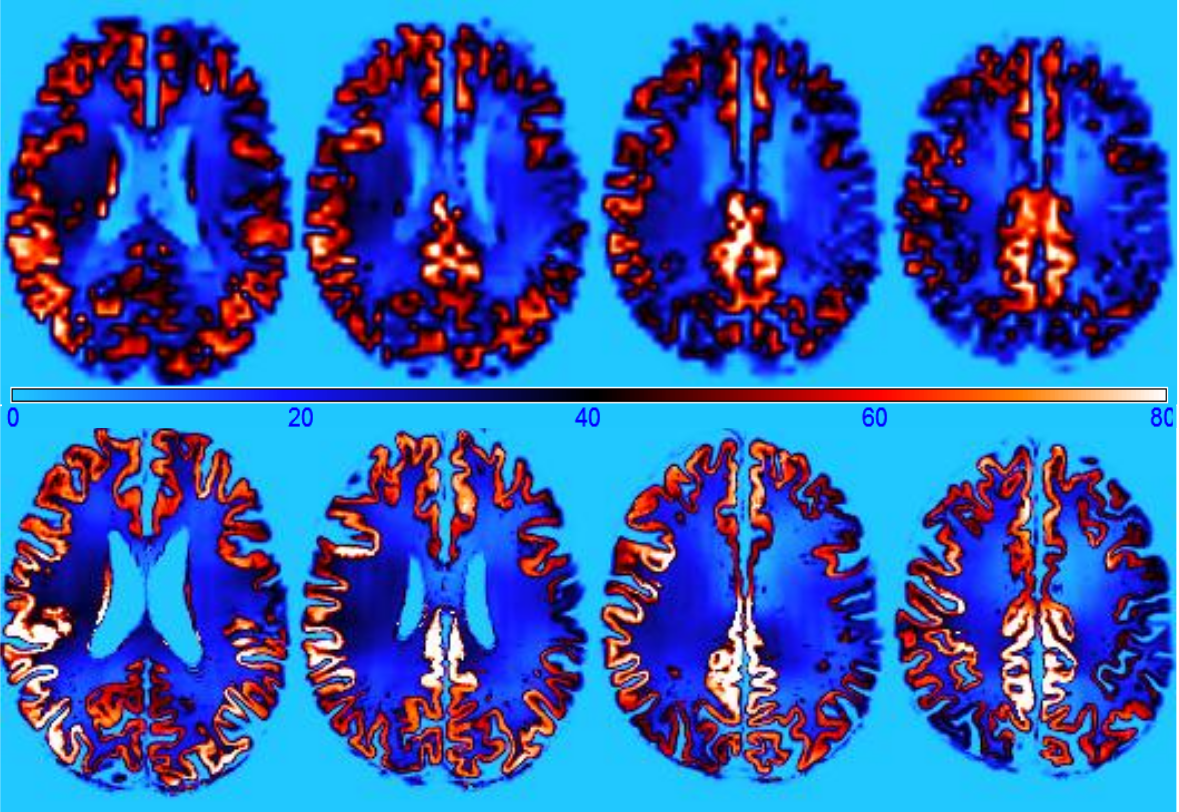
\includegraphics[width=10cm]{5_5_exemple_asllani}
\caption{Exemple d'utilisation de la correction des effets de volumes partiels d’Asllani pour améliorer
artificiellement la résolution d’une image ASL. Sur la première ligne une image d’ASL 2D normalisé via SPM
(sans lissage). En seconde ligne en normalisant les différences partielles $\Delta M_{GM}$ , $\Delta M_{WM}$  , et $\Delta M_{CSF}$ obtenues
par la méthode d’Asllani, puis en appliquant les segmentations normalisées obtenue par segmentation du $T_1$
original (1 mm isotropique) pour reconstituer l’image ASL en meilleur résolution.
}
\label{fig:5_5_exemple_asllani}	
\end{figure}
Cette méthode permet en effet de corriger efficacement les effets de volumes partiels (\cite{Asllani2008}).
Cependant, du fait de l’hypothèse de la constance de la perfusion dans les équations du kernel autour
de chaque voxel, elle induit un lissage des données. Les nouvelles méthodes d’acquisition ASL multi
temps d’inversion ont ouvert la voie à une évolution de cet algorithme. En effet, il devient possible
d’utiliser l’information contenue dans un même voxel aux différents temps d’inversion comme base
pour générer le système d’équations (\cite{Chappell2011}) de façon à avoir une solution unique sans avoir à utiliser le
kernel spatial de la méthode standard et en supprimant donc les effets de lissage.

Outre l’intérêt évident de l’approche d’Asllani dans la correction des effets de volume partiels,
il est posssible d’envisager d’autres applications une fois extrait les différences $\Delta M_{GM}$ , $\Delta M_{WM}$  , et $\Delta M_{CSF}$ {\em via} les probabilités $P_{GM}$ , $P_{WM}$ , et $P_{CSF}$ obtenues grâce à une segmentation ramenée à la résolution
de l’ASL. En effet, si comme le suppose la méthode d’Asllani la cartographie des débits partiels ne
possède que des faibles gradients dans le cerveau, elle sera moins affectée par les interpolations lors
de l’étape de normalisation qu’une image contenant de forts contrastes à petites distances. L’imagerie
$T_1$ permet de récupérer sans lissage lié à la normalisation les segmentations des tissus en haute
résolution (1 mm isotropique). Ainsi, la normalisation indépendante des différences partielles et des
segmentations du $T_1$ initial via un outil type SPM (\cite{Friston2006}) peut permettre d’améliorer la qualité de la
cartographie normalisée. L’information anatomique est portée par l’image disposant de la meilleure
résolution, l’information quantitative elle, ne subit que peu de modifications grâce aux faibles
gradients qu’elle est supposée porter. La reconstruction de la cartographie via l’Équation~\ref{eq:asllani} aboutit
ainsi à une image artificiellement mieux résolue et plus fine que la normalisation « standard » de
l’image (Figure~\ref{fig:5_5_exemple_asllani}) avec un lissage « intra-tissu ».
%%%
%%%
\section{Application CRESCENDO}
Les séquences ASL évoluent rapidement. Durant la plus grande partie de cette thèse, nous
n’avons eu accès qu’à la séquence 2D d’ASL Pulsée PICORE-Q2TIPS. Cette séquence est couramment
utilisée dans la littérature (\cite{Bastos-Leite2008},~\cite{Haller2013}) et permet d’aboutir à des résultats cohérents. Au cours de
l’acquisition une cinquantaine de répétitions sont enregistrées, qu’il est nécessaire de prétraiter afin
de corriger du mouvement, et des effets de volumes partiels précédemment évoqués, avant de
pouvoir quantifier. Nous avons donc mis en place une chaîne de traitement dédiée sous MATLAB. Pour
la valider, l’évaluer, et corriger les erreurs s’il y en a, nous l’avons appliquée à un protocole dédié à
l’analyse de la réserve cognitive chez des sujets très âgés : « CRESCENDO » (Cognitive REServe and
Clinical ENDOphenotype) (\cite{Deverdun2015}). L’objectif était d’évaluer les associations entre le débit sanguin
cérébral dans la matière grise et certains facteurs de risques cardiovasculaire sur une période de 12
ans chez des sujets âgés sains.

Les données ont été dérivées de l’étude prospective 3C de Montpellier (\cite{Alperovitch2002}] dans laquelle des
sujets âgés (âge > 65 ans) ont réalisé des évaluations standardisées et des examens cliniques à
l’inclusion (1999 – 2001) puis à 2, 4, 7, 10 et 12 ans. A 12 ans, les participants non déments ont été
invités à réaliser une IRM ainsi que des examens cliniques complémentaires dans le cadre de l’étude
CRESCENDO (n=380, 67.3 \% de femmes, âge moyen 81.96 ± 3.82 ans). Les facteurs comportementaux
tels que la consommation de cigarette et d’alcool ont été évalués à l’inclusion, l’histoire des maladies
cardiovasculaires du sujet au suivi à 12 ans. Les informations biologiques telles que le poids, la taille,
l’usage de médicaments, la glycémie, et le cholestérol sont recueillies à l’inclusion et à 10 ans. La
pression artérielle est mesurée à chaque suivi. Sur la base de ces paramètres la pression artérielle
moyenne est calculée, ainsi que les évolutions des différentes variables.

Les données IRM ont été collectées sur une IRM à 3T (Skyra, Siemens, Germany) avec une
antenne 32 éléments. Une série anatomique 3DT$_1$ a été acquise avec les paramètres suivants : champ
de vue = 25 x 25 cm, T$_E$ = 2.5 ms, T$_R$ = 1690 ms, angle de bascule = 9°, taille du voxel = 0.98 x 0.98 x 1
mm, 176 coupes. Une acquisition en inversion récupération atténuée du flux (FLAIR) a été réalisé afin
d’évaluer les lésions de la matière blanche avec les paramètres : champ de vue = 22 x 22 cm, $T_E$ = 111
ms, T$_R$ = 7000 ms, angle de bascule = 150 °, taille du voxel = 0.86 x 0.86 x 3, 39 coupes. Enfin les mesures
de débit ont été obtenues via une séquence ASL 2D pulsée, PICORE-Q2TIPS (\cite{Luh1999}), T$_{I1}$/T$_{I2}$/T$_{R}$/T$_{E}$=
700/2000/3000/20 ms, 52 répétitions, 16 coupes (1.5 mm de gap), taille du voxel = 3.44 x 3.44 x 6 mm$^3$.

L’ensemble du traitement a été réalisé sous MATLAB (MathWorks, Natick, MA) et en utilisant
SPM8 (Statistical Parametric Mapping ; The Wellcome Trust Center for Neuroimaging, UK). Toutes les
images ont été réorientées sur la commissure antérieure.

La fréquence des hypersignaux de la substance blanche augmente avec l’âge (\cite{Awad1987}). Or, du faite
de leur signal en T$_1$, ils peuvent être identifiés à tort comme de la matière grise. Sur cette cohorte il
semblait donc important de les prendre en compte. La boite à outils SPM « Lesion Segmentation Tool »
(\cite{Schmidt2012}) a donc été utilisé afin, à partir du T$_1$ et du FLAIR, d’identifier les hyper signaux de la substance
blanche et de les remplacer dans l’image T$_1$ par une valeur moyenne de la substance blanche. Cela
permet ensuite de réaliser une segmentation standard de SPM (comme décrit précédemment) sur la
base de ce T$_1$ modifié et d’obtenir les cartes de matière grise, matière blanche et liquide cérébro-
spinal. Les données d’ASL ont été réalignées sur l’image M$_0$ de la magnétisation à l’équilibre, les sujets
présentant des mouvements trop important étant éliminés. Les images marquées sont soustraites aux
images contrôle via une « surround subtraction » (Control2- (Label1+Label2)/2) afin de produire les
cartes pondérées en perfusion (\cite{Wang2008}). Enfin, les différences sont moyennées pour n’obtenir qu’une
seule image. La quantification du débit sanguin cérébral dans la matière grise est obtenue par
l’Équation~\ref{eq:debit} après correction des effets de volume partiels par méthode d’Asllani (\cite{Asllani2008}) (kernel = 7 x
7 x 1 voxels).

La vérification de la qualité des cartes de débit a mis en évidence pour un grand nombre de
sujets la présence de forts artéfacts (débits quasi-nuls sur une moitié de cerveau, forts débits dans le
liquide céphalo rachidien etc.). L’observation détaillée des cartes de perfusions de chaque répétition
a mis en évidence la présence de perfusions négatives ou nulles sur un nombre important de
répétitions pour les patients présentant ces artéfacts. Après vérification des données, cela ne semblait
pas être dû aux mouvements (les patients présentant des mouvements trop importants ayant été
retirés, n = 17). L’hypothèse la plus probable sur cette cohorte semble être le choix du temps
d’inversion. En effet, la valeur optimale de ce paramètre dépend du temps de transit du sang lui-même
dépendant de l’âge du sujet et de son histoire vasculaire. Or chez des sujets très âges cette histoire
peut fortement varier, il est donc possible que le temps choisi (temps d’inversion moyen observé dans
la littérature pour des âges similaire : 2000 ms) ne soit pas adapté à l’ensemble des sujets.

Pour détecter les patients pour lesquels les données d’ASL sont inexploitables, nous avons défini
un critère qualité :
\begin{itemize}
\item Si l’image de perfusion d’une répétition contient plus de valeurs négatives que positive, elle
est défini comme inutilisable;
\item Si le sujet dispose de plus de 20 \% de perfusions marquées comme inutilisables, il est lui-même
défini comme inexploitable.
\end{itemize}
\begin{figure}[!t]
\centering
\includegraphics[width=8cm]{5_6_qualite_asl}
\caption{Impact du temps d'inversion sur le nombre de répétitions retirées. Dans la figure A, le nombre de répétitions
retirées sur la base de notre critère est affiché pour un sujet donné et selon différents temps d’inversion. Les points noirs
correspondent aux vraies valeurs, la courbe bleue à un ajustement polynomial de second degré, la flèche rouge indique le
temps d’inversion optimal identifié sur la base de la carte de temps d’arrivé du bolus (1555 ms). La valeur minimale de la
courbe et le T$_I$ optimal semblent concordants. La figure B montre le nombre moyen de répétitions retirées pour tous les
sujets en fonction de la distance au T$_I$ optimal. La ligne rouge centrale est la moyenne, et les lignes dessus et dessous
représentent l’écart type. Lorsque la distance au T$_I$ optimal augmente, le nombre de répétitions enlevées augmente aussi. La
figure C montre les temps d’inversion optimaux des sujets (en ms) identifiés sur la base de la carte du temps d’arrivé
(« measured T$_I$ ») comparés au temps d’inversion où il y a le moins de répétitions retirées pour chaque sujet (« estimated
T$_I$ »).}
\label{fig:5_6_qualite_asl}	
\end{figure}
Pour les patients exploitables, l’analyse n’est réalisée qu’à partir des répétitions valides. C’est un
critère empirique qui permet de sélectionner les sujets et de limiter les erreurs dans l’interprétation.

Il semblait important malgré tout de s’assurer que ces artéfacts venaient bel et bien d’un mauvais
paramétrage du temps d’inversion. Pour ce faire, nous avons réalisé des acquisitions supplémentaires
sur 6 sujets sains (âge = 24.5 ± 2 ans) avec un protocole identique mais répétant l’ASL 2D en variant le
temps d’inversion (1300, 1400, 1500, 1600, 1700, 1800, 1900, et 2000 ms). Nous avons par ailleurs
rajouté une séquence obtenue récemment au sein du service : l’ASL pulsée 3D-GRASE (\cite{Gunther2005}) autorisant
le multi-T$_I$ avec les paramètres : durée du bolus = 700 ms, $T_R$ = 3000 ms, $T_E$ = 20 ms, GRAPPA 2, 24
coupes, taille du voxel = 3.4 x 3.4 x 4 mm$^3$, 16 temps d’inversion (480 à 4000 ms). Cette séquence
autorise le calcul en ligne de cartes d’arrivée du bolus ce qui permet d’évaluer le T$_I$ optimal pour le
sujet. De plus, grâce à la séquence ASL 2D on pourra évaluer le nombre de répétitions définies comme
inutilisables lorsque l’on s’éloigne du T$_I$ optimal. Si notre critère est correct, ce nombre devrait
augmenter avec l’éloignement. Un radiologue a donc extrait la durée d’arrivée du bolus pour chaque
patient en traçant une ROI dans la matière grise de différents territoires vasculaires.

La Figure~\ref{fig:5_6_qualite_asl} illustre les résultats obtenus. Comme on le voit, plus l’on s’éloigne du temps
d’inversion optimal, plus la valeur de notre critère qualité devient mauvaise (Figure~\ref{fig:5_6_qualite_asl} B et C). Par
ailleurs, le temps d’inversion optimal identifié sur la base de notre critère montre une très bonne
concordance avec les données issues des cartes des temps d’arrivés du bolus (Figure~\ref{fig:5_6_qualite_asl} C). Il semble
donc que notre hypothèse soit la bonne : le temps d’inversion n’est pas le bon pour tous les sujets.

La comparaison des caractéristiques des sujets exclus et des sujets retenues sur la base de notre
critère met en évidences des différences en termes de BMI, glycémie, âge et sexe (Tableau~\ref{tab:crescendo}). Il a été
montré que l’âge et le sexe modifient le temps de transit (\cite{Liu2012}). Les effets du BMI et de la glycémie sur
le temps de transit n’ont pas été clairement étudiés. Les sujets exclus disposent d’un BMI et d’une
glycémie plus élevée. Les hauts niveaux de glycémie induisent une augmentation de la rigidité
artérielle (\cite{Rubin2012}) ce qui impacte le temps de transit. Encore une fois ces observations sont concordantes
avec notre hypothèse sur le temps d’inversion. L’effet du BMI n’a pas été évalué dans la littérature, il
semble néanmoins au vue de ces résultats qu’il impacte le temps de transit. Au total une grande partie
des données est exclue de l’analyse, cependant assouplir le critère qualité entraine l’utilisation de
données artéfactées, et ainsi l’apparition de corrélations complètement fausses. Il est donc très
important de vérifier la qualité des données notamment chez des cohortes de sujets très âgés où le
temps d’inversion optimal peut être très variable. Par ailleurs, cela démontre l’intérêt des séquences
multi-T$_I$ chez des sujets très âgés. L'ensemble du process de sélection des données est résumé dans la figure~\ref{fig:5_7_selection_sujets}.

%%%
\begin{figure}[!t]
\centering
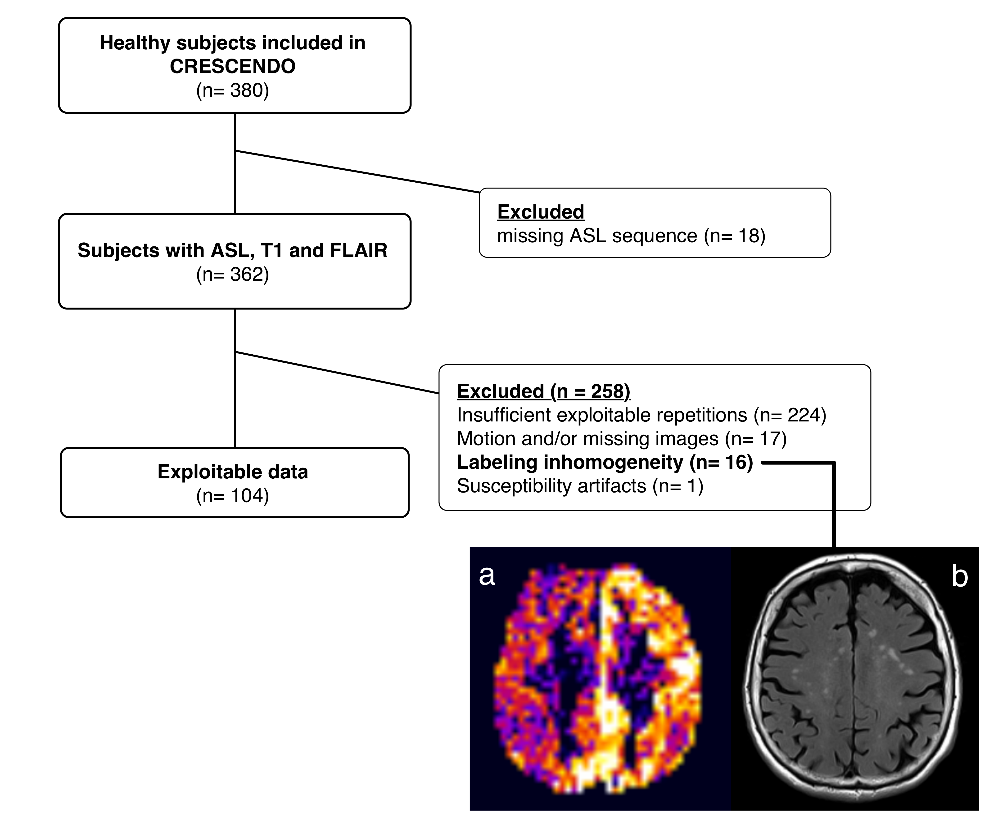
\includegraphics[width=10cm]{5_7_selection_sujets}
\caption{Diagramme décrivant la sélection des sujets. Les sujets qui ne sont pas dans les critères requis (données
manquantes, artéfactées etc.) sont exclus. Les images de perfusion ont été vérifiées et définies comme inutilisables selon le
critère qualité (n=224). Un exemple d’inhomogénéité de l’ASL est illustré avec en a) une cartographie de débit, et en b
l’image FLAIR correspondante. Alors qu’il y a une différence claire dans la carte du DSC entre les hémisphères, aucune
pathologie n’est visible en FLAIR.}
\label{fig:5_7_selection_sujets}	
\end{figure}
%%%
\begin {table}
\caption{Caractéristiques des patients de l’étude CRESCENDO retenues sur la base du critère, versus ceux exclus. A
l’inclusion, le NART, la consommation d’alcool et de cigarette ont été estimés. A 10 ans, les données biologiques (sauf le
BMI). A 12 ans, le BMI, et les facteurs de risques cardiovasculaires. Les données sont exprimées avec la moyenne et l’écart
type sauf cas contraires. Le nombre d’observations disponibles pour chaque variable est indiqué. Les différences entre les
deux groupes ont été évaluées par des tests de $\chi^2$ et des tests T.} 
\label{tab:crescendo} 
\centering
\begin{tabularx}{17cm}{X | c c c c c}
	{\em Caractéristiques } & 
	\multicolumn{2}{c}{{\em Sujets exclus}} &
	\multicolumn{2}{c}{{\em Données utilisables}} &
	{\em p-values}\\
	 & Valeur & Disponibilité & Valeur & Disponibilité & \\

	\hline
	{\em \bf Facteurs sociodémographiques } &  & & & & \\
	{\em Homme} & 134 (48,5 \%) &276 & 34 (32,7 \%) & 104 & {\bf 0.005}\\
	{\em Age, ans} & 82.25 (3,97) &276 &81,3 (3,3) &104 &{\bf 0.03}\\
	\hline
	{\em \bf Statut cognitif } &  & & & & \\
	{\em MMSE} & 28,45 (1,61)& 270 &28,78 (1,35)& 101 &{\bf 0.07}\\
	{\em NART} & 22,54 (5,77) &273 &22,28 (5,86)& 102 &{\bf 0.70}\\
	\hline
	{\em \bf Consommation d’alcool } &  & & & & \\
	{\em Aucune, n (\%)} & 34 (12,8 \%) &266 &13 (12,7 \%)& 102 &{\bf 0.57}\\
	{\em Modérée, n (\%)} & 172 (64.7 \%) &266 &71 (69,6 \%) &102 &{\bf 0.57}\\
	{\em Elevée, n (\%)} & 60 (22.6 \%) &266 &18 (17,6 \%) &102 &{\bf 0.57}\\
	\hline
	{\em \bf Consommation de cigarettes } &  & & & & \\
	{\em Non fumeur, n (\%)} & 164 (59,4 \%) &276 &70 (67,3 \%)& 104 &{\bf 0.35}\\
	{\em Ancien fumeur, n (\%)} & 93 (33,7 \%) &276 &29 (27,8 \%)& 104 &{\bf 0.35}\\
	{\em Fumeur, n (\%)} & 19 (6,9 \%) &276 &5 (4,7 \%) &104 &{\bf 0.35}\\
	\hline
	{\em \bf Données biologiques} &  & & & & \\
	{\em BMI, kg/m$^2$} & 24,72 (3,39) &274 &23,2 (2,76) &103 &{\bf <0.001}\\
	{\em $\Delta$ BMI} & 0.002 (0.08)& 265 &-0.02 (0.07) &103 &{\bf 0.008}\\
	{\em Glycémie, mmol/L} & 5,46 (0,93) &236 &5,17 (0,71) &90& {\bf 0.007}\\
	{\em $\Delta$Glyc} & -0.10 (0.16) &236 &0.08 (0.12)& 90 &{\bf <0.001}\\
	{\em Statut diabétique, n (\%)} & 43 (18 \%) &238 &13 (14,1 \%)& 92& {\bf 0.39}\\
	{\em HDL, mmol/L} & 1,55 (0,37) &235 &1,62 (0,36) &90 &{\bf 0.08}\\
	{\em LDL, mmol/L} & 3,40 (0,93) &235 &3,46 (0,88) &90 &{\bf 0.6}\\
	{\em Triglycérides, mmol/L} & 1,27 (0,52) &235 &1,20 (0,53) &90 &{\bf 0.3}\\
	{\em Cholestérol total, mmol/L} & 5,53 (1,08) &235 &5,64 (1,04) &90 &{\bf 0.41}\\
	{\em $\Delta$ Chol} & 0.04 (0.2) &235 &0.05 (0.19) &90 &{\bf 0.61}\\
	{\em Dyslipidémie, n (\%)} & 147 (60 \%)& 245 &56 (53,8 \%) &95 &{\bf 0.86}\\
	\hline
	{\em \bf Facteurs cardiovasculaires } &  & & & & \\
	{\em MAP, mmHg} & 96,73 (11) &269 &96,7 (10,9) &91 &{\bf 0.99}\\
	{\em $\Delta$ MAP} & -0.03 (1.03) &209 &0.23 (0.82) &71 &{\bf 0.05}\\
	{\em Hypertension, n (\%)} &215 (78.75 \%) &273 &75 (73 \%) &103 &{\bf 0.22}\\
	{\em Traitement HT, n (\%)} & 153 (55.64 \%) &275 &48 (46,6 \%) &103 &{\bf 0.12}\\
	{\em Maladies cardiovasculaires, n (\%)} & 67 (24.63 \%) &275 &20 (19,4 \%) &103 &{\bf 0.31}\\

\end{tabularx}

\end{table}

En vue d’appréhender les associations entre débit sanguin cérébral et données
épidémiologiques, des tests statistiques ont été réalisés. Le débit sanguin cérébral a tout d’abord été
log-transformé afin de normaliser sa distribution avant l’analyse. Les différences liées au sexe ont été
analysées via un test T de Student. Une analyse de corrélation (coefficient de corrélation de Pearson)
a été faite en vue d’examiner l’association entre l’âge et le DSC. Afin d’évaluer les associations entre
facteurs de risques cardiovasculaires ou leur évolution et DSC, des modèles de régression linaires ont
été utilisés avec ajustement sur le sexe et l’âge. Les valeurs de p inférieures à 0.0026 (0.05 corrigé des
comparaisons multiples par une correction de Bonferroni) ont été considérées comme statistiquement
significatives.

La sélection des patients exploitables a permis l’analyse des associations entres les données
épidémiologiques et le débit dans la matière grise. Le DSC moyen est de 45.2 ± 10.6 ml/100g/min. Les
résultats détaillés sont renseignés dans le Tableau~\ref{tab:crescendo2}. La comparaison des résultats avec et sans
utilisation du critère qualité met en évidence d’importantes différences en termes de significativité.
Brièvement, l’utilisation de l’ensemble de la cohorte fait apparaitre des corrélations incohérentes
telles qu’un débit élevé associé à l’atrophie corticale, de même avec l’IMC. Nous décrirons ici
uniquement les résultats obtenus après sélection des sujets.


\begin {table}
\caption{Résultats de l’analyse statistique des corrélations du DSC et de différents facteurs. Les résultats sur l’âge ont été
obtenus par une corrélation de Pearson, un test T a été utilisé pour le sexe, et une régression linéaire multivariée avec
austement sur l’âge et le sexe pour les autres variables. La significativité est indiquée par la p-value, la valeur du R$^2$ ajustée
est rapporté lorsque disponible. Les valeurs de p en gras traduisent une valeur inférieure à 0.05. Un astérix indique les valeurs
significatives après correction de Bonferroni. Les résultats sont présentés sur l’ensemble de la cohorte (sans utilisation du
critère qualité) et sur l’échantillon retenu.} 
\label{tab:crescendo2} 
\centering
\begin{tabularx}{\linewidth}{X | c c c c}
\hline
 & \multicolumn{2}{c}{{\bf Ensemble des sujets}} & \multicolumn{2}{c}{{\bf Sujets retenus}} \\
\hline
 & p-value & R$^2$ & p-value &  R$^2$\\
\hline
{\bf Age} & 0,18 & - & 0.88 & - \\
{\bf Sexe} & 0,2 & - & {\bf 0.0002$^{\ast}$} & - \\

{\bf Triglycérides} & 0,113 & 0,017 & 0.087 & 0,093\\ 
{\bf HDL} & 0,735 & 0,005 & 0,312& 0,073\\ 
{\bf LDL} & 0,084 & 0,019 & 0.202 & 0,080\\ 
{\bf Cholestérol total} & {\bf 0,044} & {\bf 0,024} & 0.243& 0,077\\ 
{\bf \'Evolution du cholesterol} & 0,593 & 0,006 & 0.690& 0,064\\ 
{\bf hypertension} & 0,057 & 0,015 & 0.734 & 0,053\\ 
{\bf diabète} & 0,353 & 0,010 & 0.534 & 0,061\\ 
{\bf Indice de masse corporelle} & {\bf 0,006} & {\bf 0,029} & 0.595 & 0,055\\ 
{\bf Pression artérielle moyenne} & 0,632 & 0,002 & 0.163 & 0,102\\ 
{\bf \'Evolution de la pression artérielle moyenne} & 0,178 & 0,010 & {\bf 0,002}$^{\ast}$& {\bf 0,210}\\ 
{\bf Atrophie corticale} & {\bf 0,002}$^{\ast}$ & {\bf 0,039} & 0.226 & 0,063\\ 
{\bf Alcool} & 0,505 & 0,003 & 0.938 & 0,052\\ 
{\bf Cigarette} & 0,382 & 0,001 & 0.603 & 0,051\\ 
{\bf Pathologies cardiovasculaires} & 0,803 & -0,002 & 0.778 & 0,053\\ 
{\bf \'Evolution de la glycémie} & 0,869 & 0,005 & 0.051 & 0,103\\ 
{\bf \'Evolution de l'indice de masse corporelle} & 0,244 & 0,004 & 0.467 & 0,057\\ 
\end{tabularx}

\end{table}

Le DSC est ainsi plus élevé chez les femmes (47.2 ± 10.8 ml/100g/min contre 41.3 ± 9.4
ml/100g/min chez les hommes). L’âge n’étant pas corrélé au DSC. De même, aucune association n’a
pu être trouvée entre la consommation de cigarette et d’alcool et le débit sanguin cérébral. L’analyse
des données sur le diabète ne révèle rien de significatif. Cependant une tendance indiquant un débit
diminué avec des hauts niveaux de glucose a été trouvé (p=0.05, R$^2$ = 0.10). De la même façon, l’analyse
des données longitudinales montre une tendance à un débit réduit lorsque la glycémie augmente
(p=0.04, R2=0.10). Il est bon de noter que les sujets retenus pour notre analyse présentent une
différence significative en termes de glycémie vis-à-vis des sujets exclus (p<0.01). Ni le cholestérol ni
la dyslipidémie, ni même les pathologies cardiovasculaires ne semblent corrélés au DSC. Alors que
l’hypertension et la pression artérielle moyenne (MAP) n’apparaissent pas associées au DSC,
l’évolution de la pression artérielle moyenne l’est. En effet, une augmentation de la MAP sur 12 ans
est associée à un débit plus faible (p<0.003, R$^2$=0.21).

Les différences d’associations après utilisation des données de l’ensemble de la cohorte et de
l’échantillon retenu sur la base du critère qualité mettent en évidence des corrélations incohérentes.
Le résultat le plus significatif (évolution de la pression artérielle moyenne) aurait été masqué par la
présence de données complètement artéfactées du fait d’un choix du temps d’inversion non adapté à
chaque sujet. Cela montre l’importance de ce critère.

Les débits perfusionnels mesurés correspondent aux résultats attendus (\cite{Chen2011},~\cite{Brumm2010}). Nos
résultats montrent que parmi les facteurs de risques cardiovasculaires, l’évolution de la pression
artérielle moyenne est fortement associée au DSC, ce qui n’avait jamais été décrit. Or ni l’hypertension
ni la pression artérielle au moment de l’IRM n’est associé au DSC. Afin de maintenir un débit constant
malgré les variations de MAP, le cerveau adapte sa vascularisation via divers mécanismes connues sous
le nom d’autorégulation cérébrale (\cite{Paulson1990}). L’absence d’association entre CBF et MAP tend à montrer que
ce mécanisme est préservé chez les sujets âgés sains, ce qui a été évoqué chez des cohortes plus jeunes
(\cite{Vanbeek2008}). Plutôt que la MAP au moment de l’IRM, il semble que ce soit son évolution sur 12 ans ($\Delta$ MAP)
qui a le plus d’effet sur le DSC.

La courbe d’autorégulation cérébrale est capable de se décaler de façon réversible vers la
droite en cas d’hypertension chronique (\cite{Traon2002}, voir figure~\ref{fig:5_8_autoregulation}). Nos résultats suggèrent l’existence d’un
décalage vertical, inversement associé à l’évolution à long terme de la MAP. Les sujets âgés présentent
un DSC plus faible que les jeunes ce qui peut être vue comme un décalage vers le bas de la courbe avec
l’âge. Nous avons trouvé qu’une diminution de la MAP est corrélée à un débit élevé. Ces résultats sont
compatibles avec le fait que lorsque la MAP est restaurée à des valeurs plus faible, le DSC revient à des
valeurs proches de celui de personnes plus jeunes. Inversement, l’augmentation de la MAP semble
être relié à un décalage vers le bas de la courbe d’autorégulation, et donc à une réduction du débit
sanguin.\\
%%%
\begin{figure}[!t]
\centering
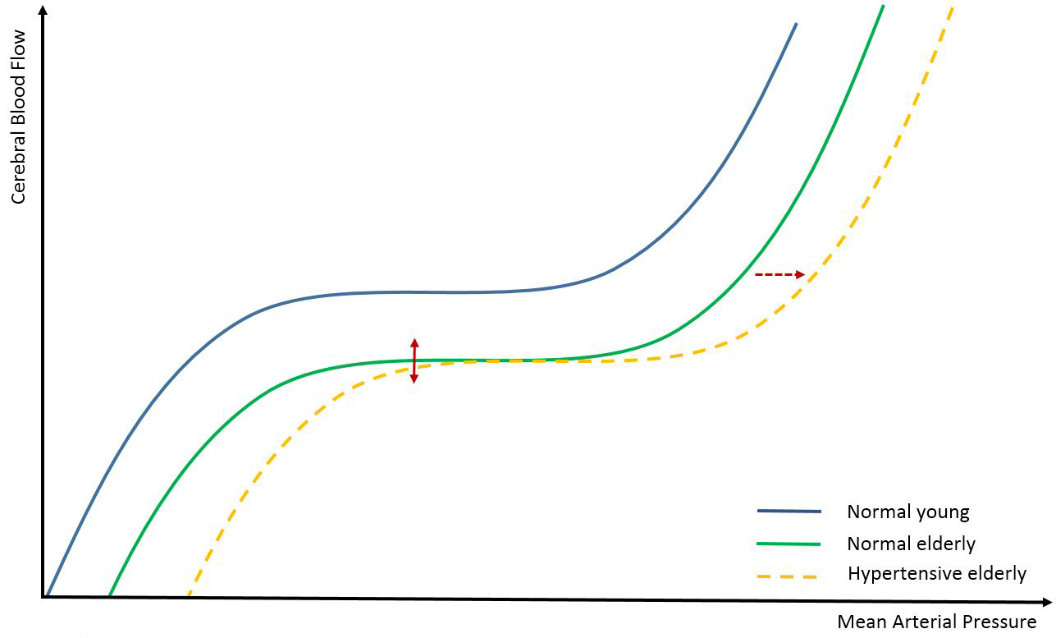
\includegraphics[width=10cm]{5_8_autoregulation}
\caption{Courbe théorique de l'autorégulation dans différents contextes. La courbe théorique chez les sujets normotensifs
jeunes est indiquée en bleu, chez les sujets normotensifs âgés en vert, et chez les sujets hypertensifs chroniques en pointillés
jaune. Les sujets âgés ont un débit sanguin cérébral plus faible que les plus jeunes, la flèche en pointillés rouge indique le
décalage vers la droite de la courbe dans le cadre de l’hypertension chronique. La double flèche rouge met en évidence la
capacité de la courbe à se décaler verticalement en fonction de l’évolution à long terme de la pression artérielle moyenne
chez les sujets âgés.}
\label{fig:5_8_autoregulation}	
\end{figure}
Les études précédentes ont suggéré cette relation entre le DSC et l’évolution de la MAP chez
des sujets âgés avec des traitements intensifs de réduction de la pression sanguine (\cite{Tryambake2013}). Nos données
indiquent que les observations obtenues à partir de traitements intensifs se produisent aussi en
conditions standard mais avec des délais plus longs. Il est important de noter que l’évolution de la MAP
peut être un effet des traitements anti-hypertensif. Cependant, dans notre cohorte moins d’un tiers
de nos sujets ont commencé un traitement durant l’étude, et aucun des patients traité n’a arrêté son
traitement. Nous avons testé les différences d’évolution entre les sujets « stables » (sur la base du
traitement) et les nouveaux traités mais nous n’avons pas été en mesure de mettre en évidence une
quelconque différence d’évolution (t-test, p = 0.72).

Un DSC réduit chez les hommes a déjà été établit chez les sujets âgés (\cite{Liu2012},~\cite{Chen2011}). Nos résultats
confirment ces observations. Parmi les explications possibles, on notera un taux d’hématocrite plus
faible chez les femmes (\cite{Liu2012}). Ces effets apparaissent globaux, il est ainsi important de prendre en
compte cette variable en tant que facteur confondant dans les études de DSC. Les hommes ont une
espérance de vie plus courte que les femmes et il a été montré qu’un débit plus faible est associé à un
risque accru de mortalité de toute cause (\cite{Sabayan2013}).

Comme le sexe, l’effet de l’âge sur le DSC est bien documenté. Une diminution du débit est
observé avec l’âge en ASL et en tomographie par émission de positons (\cite{Chen2011},~\cite{Martin1991}). Nous n’avons mis
en évidence aucune association entre l’âge et le DSC dans notre cohorte. Ce résultat peut être dû à
l’homogénéité en âge dans la cohorte empêchant l’observation de cette association.

Le diabète réduit la réactivité cérébrovasculaire (\cite{Dandona1978},~\cite{Fulesdi1997}). L’absence d’association entre les
diabètes de type 2 et le DSC peut être un problème de puissance avec seulement 13 cas de diabètes
de ce type. Les niveaux de glycémie et leurs évolutions, bien que non significatif après correction de
Bonferroni, montrent une tendance négative avec le DSC. Cette observation est en adéquation avec
les données de la littérature dans lesquelles une augmentation de la rigidité artérielle a été observée
dans les cas d’hyperglycémies (\cite{Rubin2012}).

Dans les études précédentes, un débit réduit a été observé avec l’augmentation de l’indice de
masse corporelle (\cite{Willeumier2011}), la consommation chronique d’alcool (\cite{Schmidt2012}) et la consommation de cigarette
(\cite{Kubota1983}). Nous n’avons pas pu mettre en évidence de telles associations. L’explication est certainement
que, comme l’âge, leur gamme de valeur dans notre échantillon est très faible. L’intervalle de deux ans
entre la récupération des données biologiques et l’IRM doit aussi être gardé à l’esprit, et représente
une limitation pour nos conclusions.

Enfin, aucune association claire entre les évènements cardiovasculaires et le DSC n’a été
trouvée. Il est indispensable néanmoins de de se souvenir que le recrutement de nos sujets sélectionne
en soi une population « saine ». En effet, la prévalence des évènements cardiovasculaires dans notre
groupe est bien en dessous de la moyenne pour des sujets de cet âge.

La force de cette étude réside dans la disponibilité des cartographies des débits sanguins
cérébraux pour un nombre inhabituellement important de sujets très âgés avec les données
sociodémographiques et cardiovasculaires sur 12 ans. Nos résultats montrent à la fois l’importance de
la vérification de la qualité des données ASL, mais met aussi en évidence un phénomène non décrit à
l’heure actuelle : la capacité de la courbe d’autorégulation à se décaler verticalement en fonction de l’évolution de la pression artérielle moyenne. Plus que la valeur de la pression artérielle moyenne, son
évolution semble donc être un paramètre important à surveiller chez les personnes âgées.

































\bibliography{jeremythesebib}{}
\bibliographystyle{francaissc}